% 东北大学博士学位论文 LaTeX 模板（2026 版）
\documentclass[blindreview=false]{neudissertation}

\neudisetup{
  classification = {},
  security-level = {},
  udc = {},
  student-id = {},
  title-cn = {面向机械翻译的随机词汇语义驱动方法的研究},
  title-en = {Machine Translation Orented Stochastic\\Lexical Semantic Driven Approach},
  author-cn = {李某某},
  author-en = {Li Mou},
  college-cn = {计算机科学与工程学院},
  major-cn = {计算机软件与理论},
  major-en = {Computer Software and Theory},
  degree-level = {博士},
  discipline = {},
  supervisor-cn = {张某某},
  supervisor-title-cn = {教授},
  supervisor-affiliation-cn = {东北大学计算机科学与工程学院},
  supervisor-en = {Professor Zhang Moumou},
  cosupervisor-cn = {},
  cosupervisor-title-cn = {},
  cosupervisor-affiliation-cn = {},
  cosupervisor-en = {},
  submit-date = {2016年4月},
  defense-date = {2016年6月},
  degree-date = {2016年7月},
  defense-chair = {王某某},
  cover-date-cn = {2016年7月},
  cover-date-en = {January 2016},
  online-release = {两年},
  signature-date = {},
  author-signature = {Figures/signature.jpeg},
  supervisor-signature = {Figures/signature.jpeg},
  signature-height = {8mm}
}

% 用户扩展宏包
\usepackage{algorithm}
\usepackage{algorithmic}
\usepackage{makecell}
\usepackage{lipsum}
\usepackage{zhlipsum}

\begin{document}

\makeneucovers

\frontmatter

\makeneudeclaration

\begin{abstract-cn}
  跨越语言的障碍，实现不同语言人们之间的自由交流，是人类自古以来的一个梦想。机器翻译理论的研究目的在于应用计算机作为智能处理工具，实现异种自然语言间的自动翻译过程，其技术意义和社会意义都是十分深远的。

然而由于自然语言的复杂性，直至今天机器翻译的研究仍面临着巨大的困难。除词汇歧义和转换变异映射外，结构歧义一直是机器翻译研究中的主要困难之一。这是因为，各种机器翻译方法，无论是基于知识的还是基于经验的，都或多或少地依赖于源语的结构标注信息来完成语言的转换生成过程。


\cnkeywords{自然语言处理；词汇语义驱动；结构消歧；机器翻译；随机语言模型；知识获取}
\end{abstract-cn}

\begin{enabstract}
  \input{enabstract}
\end{enabstract}

\tableofcontents

\mainmatter

%!TEX root = ./main.tex
\chapter{论文格式样例与模板验证}

本章作为模板的集中样例章，用于快速检查正文中常见排版元素的显示效果。
样例覆盖章节层级、正文段落、列表、脚注、图、表、公式、算法、交叉引用和参考文献引用等内容。
编写正式论文时，可以保留本章作为排版对照，也可以删除本章并从第~\ref{chap:introduction}~章开始撰写正文。

\section{章节层级与正文段落}

论文正文通常从一级标题开始组织内容，一级标题使用 \verb|\chapter|，二级标题使用 \verb|\section|，三级标题使用 \verb|\subsection|。
本模板会自动设置章标题、节标题、页眉、页码和目录格式，作者只需要关注正文内容。
正文段落首行缩进、行距和中英文字体均由模板统一控制。

中文正文可以直接书写；英文术语建议在首次出现时给出全称，例如自然语言处理（Natural Language Processing, NLP）。
行内公式可以写作 $E=mc^2$，行内代码或命令可以使用 \verb|\verb|，例如 \verb|%!TEX root = ./main.tex
\chapter{论文格式样例与模板验证}

本章作为模板的集中样例章，用于快速检查正文中常见排版元素的显示效果。
样例覆盖章节层级、正文段落、列表、脚注、图、表、公式、算法、交叉引用和参考文献引用等内容。
编写正式论文时，可以保留本章作为排版对照，也可以删除本章并从第~\ref{chap:introduction}~章开始撰写正文。

\section{章节层级与正文段落}

论文正文通常从一级标题开始组织内容，一级标题使用 \verb|\chapter|，二级标题使用 \verb|\section|，三级标题使用 \verb|\subsection|。
本模板会自动设置章标题、节标题、页眉、页码和目录格式，作者只需要关注正文内容。
正文段落首行缩进、行距和中英文字体均由模板统一控制。

中文正文可以直接书写；英文术语建议在首次出现时给出全称，例如自然语言处理（Natural Language Processing, NLP）。
行内公式可以写作 $E=mc^2$，行内代码或命令可以使用 \verb|\verb|，例如 \verb|%!TEX root = ./main.tex
\chapter{论文格式样例与模板验证}

本章作为模板的集中样例章，用于快速检查正文中常见排版元素的显示效果。
样例覆盖章节层级、正文段落、列表、脚注、图、表、公式、算法、交叉引用和参考文献引用等内容。
编写正式论文时，可以保留本章作为排版对照，也可以删除本章并从第~\ref{chap:introduction}~章开始撰写正文。

\section{章节层级与正文段落}

论文正文通常从一级标题开始组织内容，一级标题使用 \verb|\chapter|，二级标题使用 \verb|\section|，三级标题使用 \verb|\subsection|。
本模板会自动设置章标题、节标题、页眉、页码和目录格式，作者只需要关注正文内容。
正文段落首行缩进、行距和中英文字体均由模板统一控制。

中文正文可以直接书写；英文术语建议在首次出现时给出全称，例如自然语言处理（Natural Language Processing, NLP）。
行内公式可以写作 $E=mc^2$，行内代码或命令可以使用 \verb|\verb|，例如 \verb|\input{chapter0-guide}|。
脚注示例如此处所示\footnote{脚注用于补充说明，不宜放置过长的正文内容。}。

\subsection{字体、字号与强调}

模板预定义了常用中文字体命令。正式论文中通常不需要手动切换字体；只有在展示样式、术语强调或特殊说明时才建议使用。
需要注意的是，Windows 常用中文字体多数只有常规字重，没有独立的粗体字形。
因此 \verb|\bfseries| 或 \verb|\textbf| 对宋体、黑体、楷体、仿宋等中文字体未必产生真正加粗效果；模板中的黑体标题主要依靠“黑体”本身的笔画风格，而不是额外叠加粗体。
若需要强调中文内容，建议优先使用黑体、调整标题层级或通过文字表述强调，不建议依赖中文伪粗体。

\begin{table}[H]
  \centering
  \twotabcaption{tab:ch0-fonts}{字体与强调样例}{Examples of Fonts and Emphasis}
  \begin{tabular}{lll}
    \toprule
    命令 & 显示效果 & 使用建议 \\
    \midrule
    \verb|\song| & {\song 宋体文字示例} & 正文默认字体 \\
    \verb|\hei| & {\hei 黑体文字示例} & 标题或强调场景 \\
    \verb|\kai| & {\kai 楷体文字示例} & 摘要、题签或引用语 \\
    \verb|\fs| & {\fs 仿宋文字示例} & 特殊文书类内容 \\
    \verb|\textbf| & \textbf{加粗文字示例} & 主要用于英文、数字或有粗体字重的字体 \\
    \verb|\textit| & \textit{Italic text example} & 英文斜体或变量说明 \\
    \bottomrule
  \end{tabular}
\end{table}

\subsection{列表环境}

无序列表适合列出并列事项：
\begin{itemize}
  \item 图题位于图下方，表题位于表上方。
  \item 图表应使用中英文双语标题。
  \item 公式、图、表、算法均应使用标签进行交叉引用。
\end{itemize}

有序列表适合描述步骤：
\begin{enumerate}
  \item 在 \texttt{main.tex} 中填写论文元信息。
  \item 在各章文件中撰写正文内容。
  \item 使用 \texttt{latexmk -xelatex main.tex} 完成编译。
\end{enumerate}

\section{图形排版}

本模板提供 \verb|\twofigcaption{label}{中文题名}{English title}| 用于生成中英文图题。
图题应置于图形下方，正文中使用 \verb|\figref{label}| 引用。

\subsection{外部图片}
\begin{figure}[H]
  \centering
  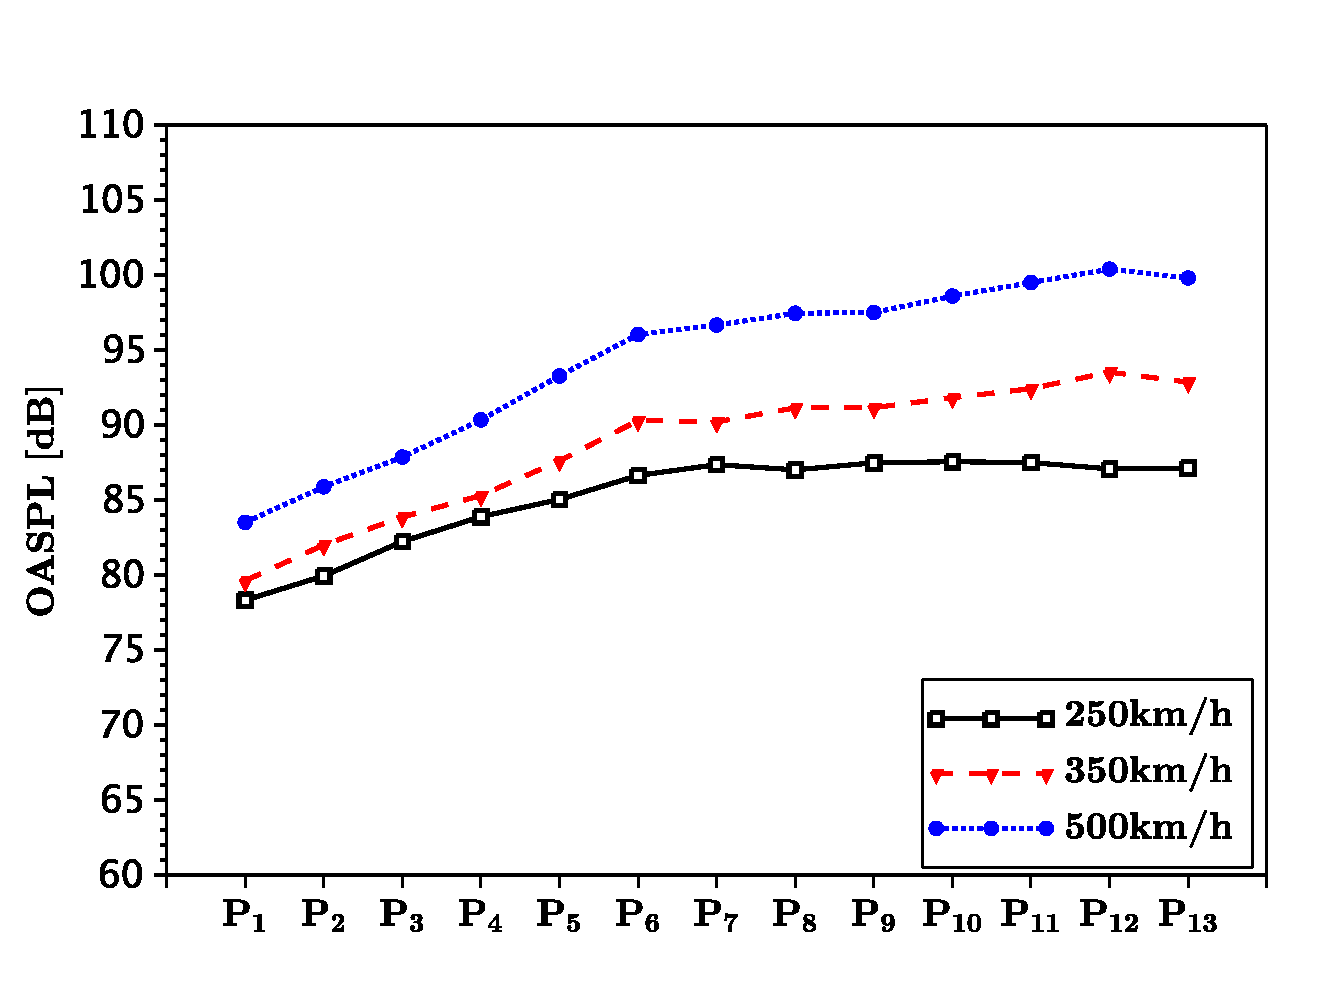
\includegraphics[width=0.55\textwidth]{Figures/oaspl_a.pdf}
  \twofigcaption{fig:ch0-cover}{外部图片插入样例}{Example of Including an External Image}
\end{figure}

\figref{fig:ch0-cover} 展示了通过 \verb|\includegraphics| 插入图片文件的方式。
正式论文中建议将图片统一放入 \texttt{Figures} 目录，并使用相对路径引用。

\subsection{PDF 或位图图片}
\begin{figure}[H]
  \centering
  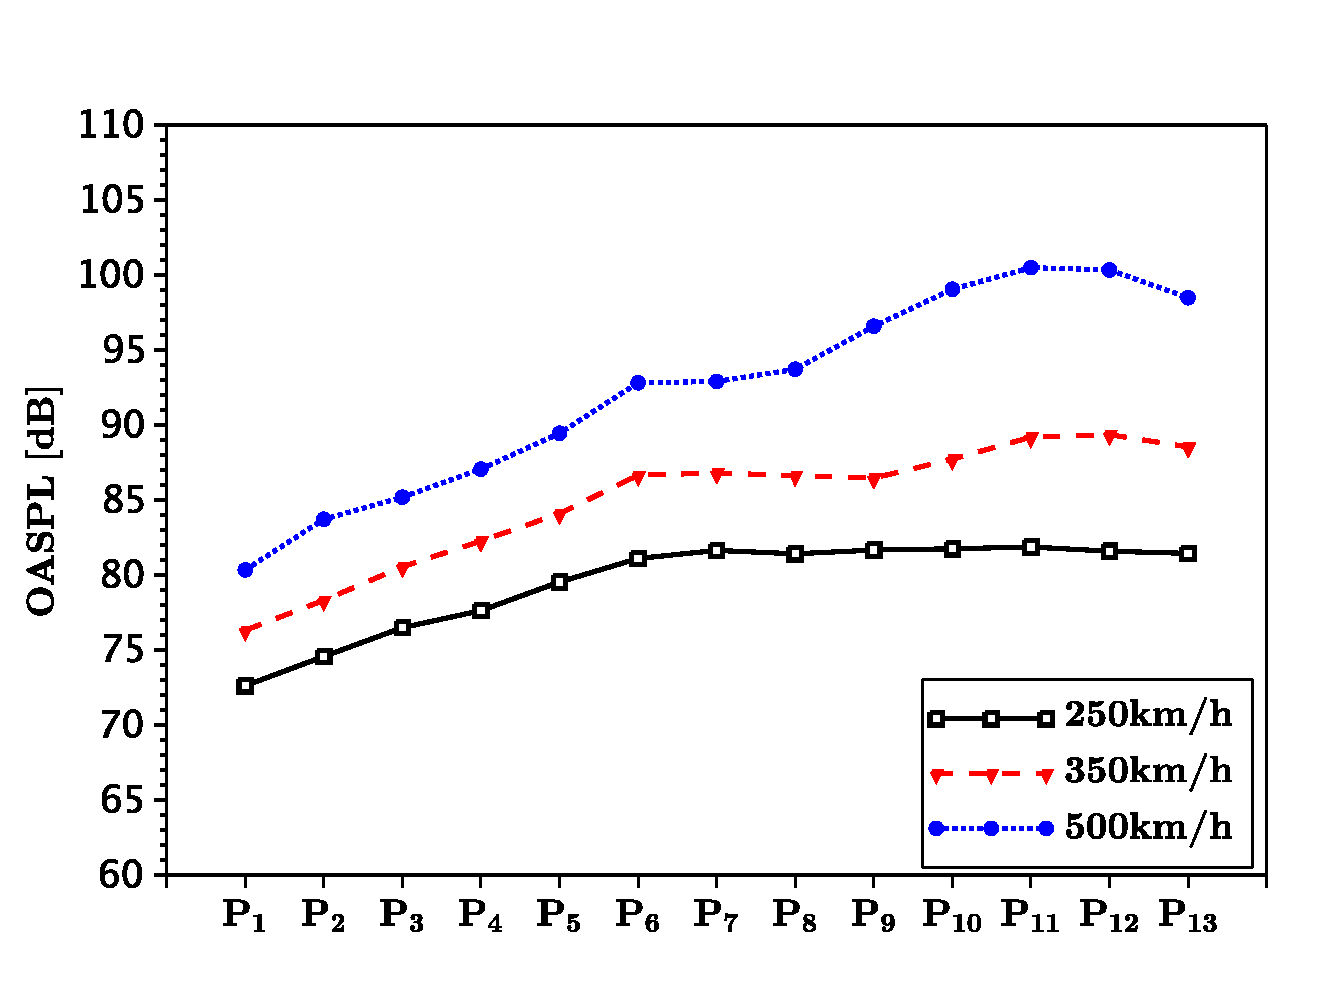
\includegraphics[width=0.55\textwidth]{Figures/oaspl_b.pdf}
  \twofigcaption{fig:ch0-pdf}{PDF 图片插入样例}{Example of Including a PDF Figure}
\end{figure}

PDF、PNG、JPG 等常见图片格式均可通过 \verb|\includegraphics| 插入。
若图片由绘图软件或数据分析程序导出，建议优先使用 PDF 格式以保持较清晰的显示效果。

\subsection{并列图片}
\begin{figure}[H]
  \centering
  \begin{minipage}[t]{0.46\linewidth}
    \centering
    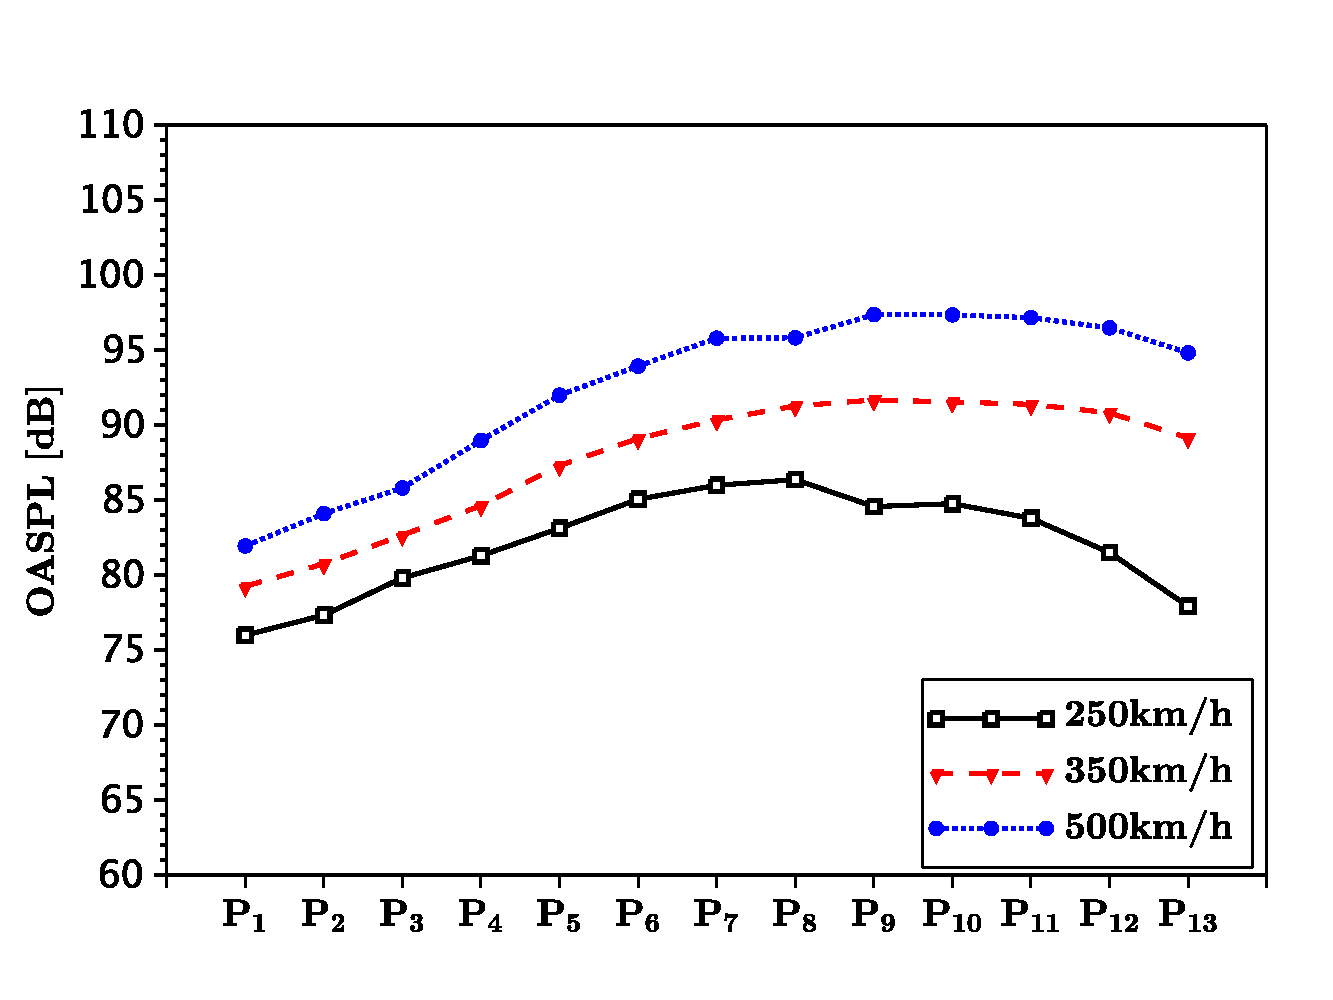
\includegraphics[width=\linewidth]{Figures/oaspl_c.pdf}
  \end{minipage}
  \hfill
  \begin{minipage}[t]{0.46\linewidth}
    \centering
    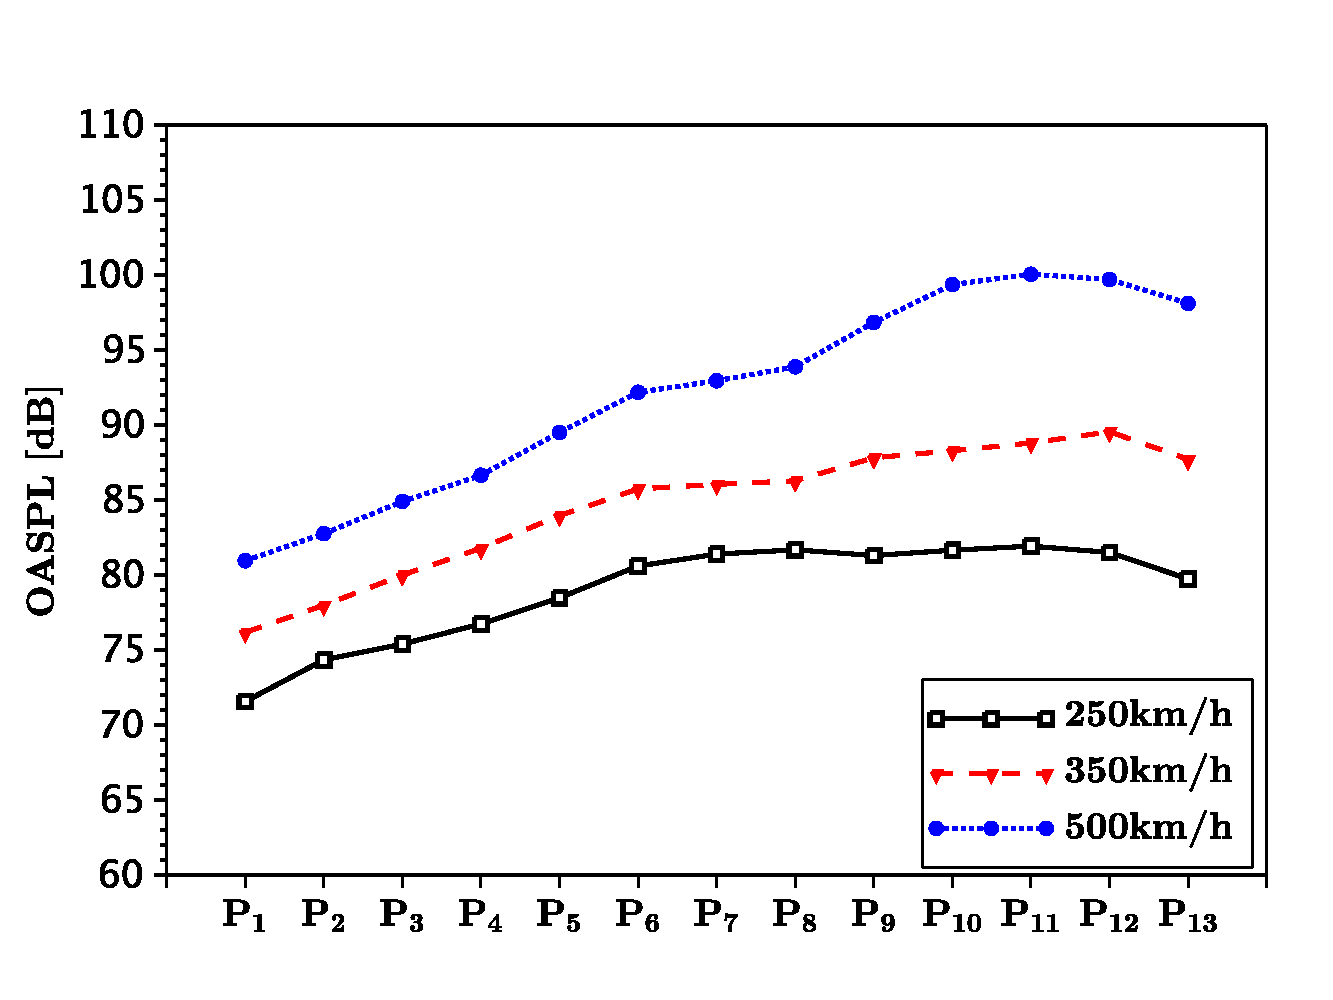
\includegraphics[width=\linewidth]{Figures/oaspl_d.pdf}
  \end{minipage}
  \twofigcaption{fig:ch0-side-by-side}{并列图形排版样例}{Example of Side-by-Side Figures}
\end{figure}

\figref{fig:ch0-side-by-side} 使用 \texttt{minipage} 完成并列排版。
当两幅图共享一个总标题时，可使用这种方式；如果每幅图都需要独立编号，建议拆成两个独立的 \texttt{figure} 环境。

\section{表格排版}

本模板提供 \verb|\twotabcaption{label}{中文题名}{English title}| 用于生成中英文表题。
表题应置于表格上方，正文中使用 \verb|\tabref{label}| 引用。

\subsection{三线表}

文本测试A

\begin{table}[H]
  \centering
  \twotabcaption{tab:ch0-booktabs}{三线表样例}{Example of a Three-Line Table}
  \begin{tabular}{lccc}
    \toprule
    方法 & 准确率（\%） & 召回率（\%） & F1 值 \\
    \midrule
    Baseline & 85.2 & 84.1 & 0.846 \\
    Method A & 89.7 & 88.9 & 0.893 \\
    Proposed & \textbf{92.1} & \textbf{91.5} & \textbf{0.918} \\
    \bottomrule
  \end{tabular}
\end{table}

\tabref{tab:ch0-booktabs} 展示了推荐的三线表格式。
论文中应尽量避免过多竖线，以保持表格简洁。

\subsection{复杂表格}
\begin{table}[H]
  \centering
  \twotabcaption{tab:ch0-complex}{合并单元格与自动换行表格样例}{Example of Merged Cells and Auto-Wrapping Columns}
  \begin{tabularx}{\textwidth}{llXc}
    \toprule
    类别 & 指标 & 说明 & 是否必需 \\
    \midrule
    \multirow{2}{*}{图形} & 分辨率 & 位图图片应保证在最终 PDF 中清晰可辨。 & 是 \\
    & 题名 & 图题使用中英文双语标题，并位于图片下方。 & 是 \\
    \midrule
    \multirow{2}{*}{表格} & 宽度 & 宽表格可使用 \texttt{tabularx} 自动分配列宽。 & 否 \\
    & 表注 & 表内说明应简明，必要时可在正文中解释。 & 否 \\
    \bottomrule
  \end{tabularx}
\end{table}

\tabref{tab:ch0-complex} 同时展示了 \verb|\multirow|、\verb|\makecell| 可配合使用的复杂表格场景。
若单元格内容较长，优先使用 \texttt{tabularx} 或 \texttt{p\{...\}} 列类型控制宽度。

\section{公式排版}

公式应使用标准数学环境，并通过 \verb|\label| 设置标签。
引用公式时建议使用模板提供的 \verb|\equref{label}|。

\subsection{单行公式}
以分类任务中的交叉熵损失为例，可写为
\begin{equation}
  \mathcal{L}(\theta)
  = - \frac{1}{N}\sum_{i=1}^{N}\sum_{k=1}^{K} y_{ik}\log p_{ik}
  \label{eq:ch0-loss}
\end{equation}

如 \equref{eq:ch0-loss} 所示，带编号公式适合放置正文中需要引用的重要定义。

\subsection{多行公式}
循环模型中的状态更新和输出计算可写为
\begin{align}
  h_t &= \sigma(W_x x_t + W_h h_{t-1} + b), \label{eq:ch0-state} \\
  \hat{y}_t &= \operatorname{softmax}(W_o h_t). \label{eq:ch0-output}
\end{align}

\equref{eq:ch0-state} 和 \equref{eq:ch0-output} 展示了多行公式的编号方式。
如果多行推导只需要一个编号，可使用 \texttt{aligned} 放在 \texttt{equation} 环境内部。

\subsection{分段函数与矩阵}
分段函数和矩阵经常同时出现在数学定义中，例如
\begin{equation}
  g(x)=
  \begin{cases}
    0, & x < 0, \\
    x, & 0 \le x < 1, \\
    1, & x \ge 1,
  \end{cases}
  \qquad
  A =
  \begin{bmatrix}
    1 & 0 & 0 \\
    0 & 1 & 0 \\
    0 & 0 & 1
  \end{bmatrix}.
  \label{eq:ch0-piecewise}
\end{equation}

\equref{eq:ch0-piecewise} 展示了分段函数和矩阵的常见写法。

\section{算法伪代码}

计算机类论文常需要给出算法步骤。本文档在 \texttt{main.tex} 中加载了 \texttt{algorithm} 和 \texttt{algorithmic} 宏包，可以直接使用如下环境。

\begin{algorithm}[H]
  \caption{样例训练流程}
  \label{alg:ch0-training}
  \begin{algorithmic}[1]
    \REQUIRE Training set $\mathcal{D}$, learning rate $\eta$, maximum epoch $T$
    \ENSURE Model parameters $\theta$
    \STATE Initialize parameters $\theta$
    \FOR{$t = 1$ to $T$}
      \STATE Sample a mini-batch $\mathcal{B}$ from $\mathcal{D}$
      \STATE Compute loss $\mathcal{L}(\theta)$ by \equref{eq:ch0-loss}
      \STATE Update $\theta \leftarrow \theta - \eta \nabla_{\theta}\mathcal{L}(\theta)$
    \ENDFOR
    \RETURN $\theta$
  \end{algorithmic}
\end{algorithm}

算法~\ref{alg:ch0-training} 展示了带行号的伪代码。
若需要中文关键字，可在导言区重定义相应命令。

\section{引用、链接与交叉引用}

参考文献引用可使用两种方式：
上标引用适合放在句末，例如已有研究讨论了神经网络轻量化问题\upcite{guo_2023_research}；
正文引用适合作为句子成分，例如文献 \inlinecite{thakkar_2018_performance} 给出了系统性能评测案例。
多篇文献可写在同一条引用命令中，例如区块链平台相关研究\upcite{zheng_2019_nutbaas,thakkar_2018_performance}。

交叉引用建议统一使用模板命令：
\begin{itemize}
  \item 图引用：\verb|\figref{fig:ch0-pdf}|，效果为 \figref{fig:ch0-pdf}。
  \item 表引用：\verb|\tabref{tab:ch0-complex}|，效果为 \tabref{tab:ch0-complex}。
  \item 公式引用：\verb|\equref{eq:ch0-loss}|，效果为 \equref{eq:ch0-loss}。
  \item 算法引用：当前模板未单独封装算法引用命令，可写作“算法~\ref{alg:ch0-training}”。
\end{itemize}
|。
脚注示例如此处所示\footnote{脚注用于补充说明，不宜放置过长的正文内容。}。

\subsection{字体、字号与强调}

模板预定义了常用中文字体命令。正式论文中通常不需要手动切换字体；只有在展示样式、术语强调或特殊说明时才建议使用。
需要注意的是，Windows 常用中文字体多数只有常规字重，没有独立的粗体字形。
因此 \verb|\bfseries| 或 \verb|\textbf| 对宋体、黑体、楷体、仿宋等中文字体未必产生真正加粗效果；模板中的黑体标题主要依靠“黑体”本身的笔画风格，而不是额外叠加粗体。
若需要强调中文内容，建议优先使用黑体、调整标题层级或通过文字表述强调，不建议依赖中文伪粗体。

\begin{table}[H]
  \centering
  \twotabcaption{tab:ch0-fonts}{字体与强调样例}{Examples of Fonts and Emphasis}
  \begin{tabular}{lll}
    \toprule
    命令 & 显示效果 & 使用建议 \\
    \midrule
    \verb|\song| & {\song 宋体文字示例} & 正文默认字体 \\
    \verb|\hei| & {\hei 黑体文字示例} & 标题或强调场景 \\
    \verb|\kai| & {\kai 楷体文字示例} & 摘要、题签或引用语 \\
    \verb|\fs| & {\fs 仿宋文字示例} & 特殊文书类内容 \\
    \verb|\textbf| & \textbf{加粗文字示例} & 主要用于英文、数字或有粗体字重的字体 \\
    \verb|\textit| & \textit{Italic text example} & 英文斜体或变量说明 \\
    \bottomrule
  \end{tabular}
\end{table}

\subsection{列表环境}

无序列表适合列出并列事项：
\begin{itemize}
  \item 图题位于图下方，表题位于表上方。
  \item 图表应使用中英文双语标题。
  \item 公式、图、表、算法均应使用标签进行交叉引用。
\end{itemize}

有序列表适合描述步骤：
\begin{enumerate}
  \item 在 \texttt{main.tex} 中填写论文元信息。
  \item 在各章文件中撰写正文内容。
  \item 使用 \texttt{latexmk -xelatex main.tex} 完成编译。
\end{enumerate}

\section{图形排版}

本模板提供 \verb|\twofigcaption{label}{中文题名}{English title}| 用于生成中英文图题。
图题应置于图形下方，正文中使用 \verb|\figref{label}| 引用。

\subsection{外部图片}
\begin{figure}[H]
  \centering
  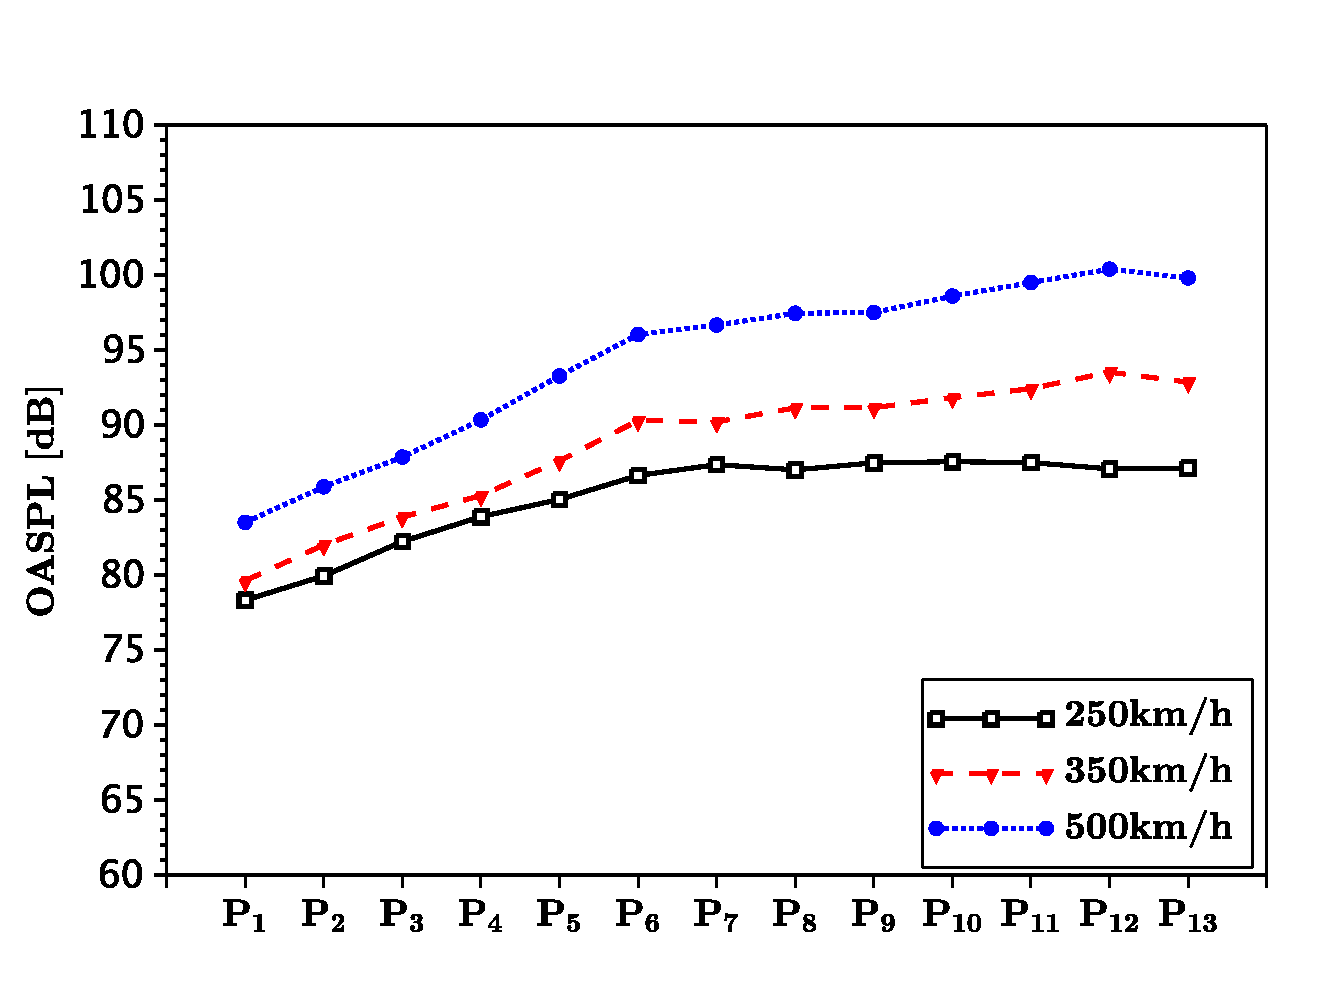
\includegraphics[width=0.55\textwidth]{Figures/oaspl_a.pdf}
  \twofigcaption{fig:ch0-cover}{外部图片插入样例}{Example of Including an External Image}
\end{figure}

\figref{fig:ch0-cover} 展示了通过 \verb|\includegraphics| 插入图片文件的方式。
正式论文中建议将图片统一放入 \texttt{Figures} 目录，并使用相对路径引用。

\subsection{PDF 或位图图片}
\begin{figure}[H]
  \centering
  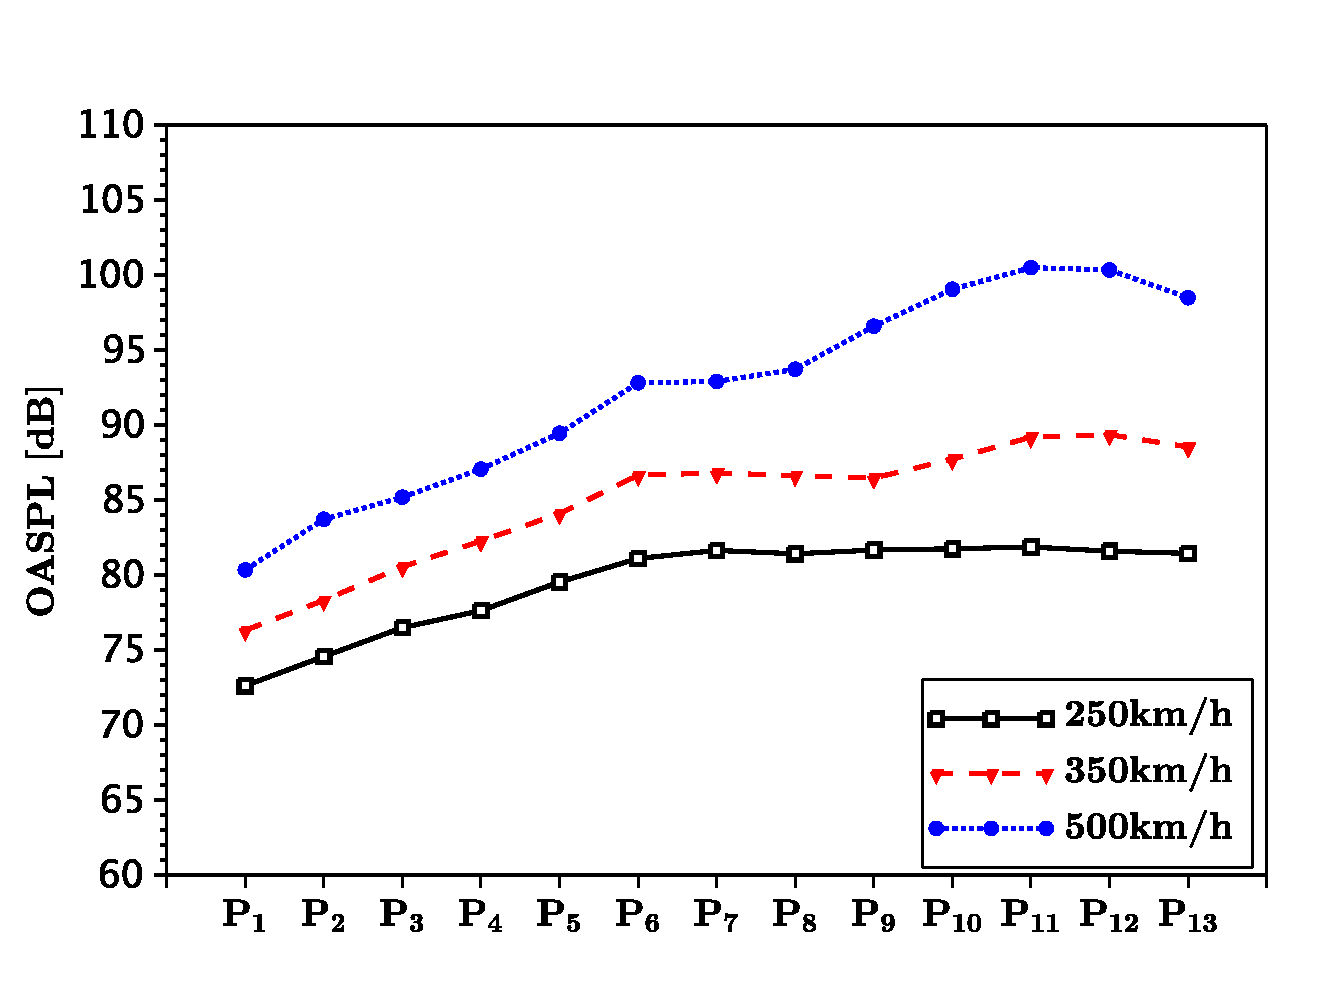
\includegraphics[width=0.55\textwidth]{Figures/oaspl_b.pdf}
  \twofigcaption{fig:ch0-pdf}{PDF 图片插入样例}{Example of Including a PDF Figure}
\end{figure}

PDF、PNG、JPG 等常见图片格式均可通过 \verb|\includegraphics| 插入。
若图片由绘图软件或数据分析程序导出，建议优先使用 PDF 格式以保持较清晰的显示效果。

\subsection{并列图片}
\begin{figure}[H]
  \centering
  \begin{minipage}[t]{0.46\linewidth}
    \centering
    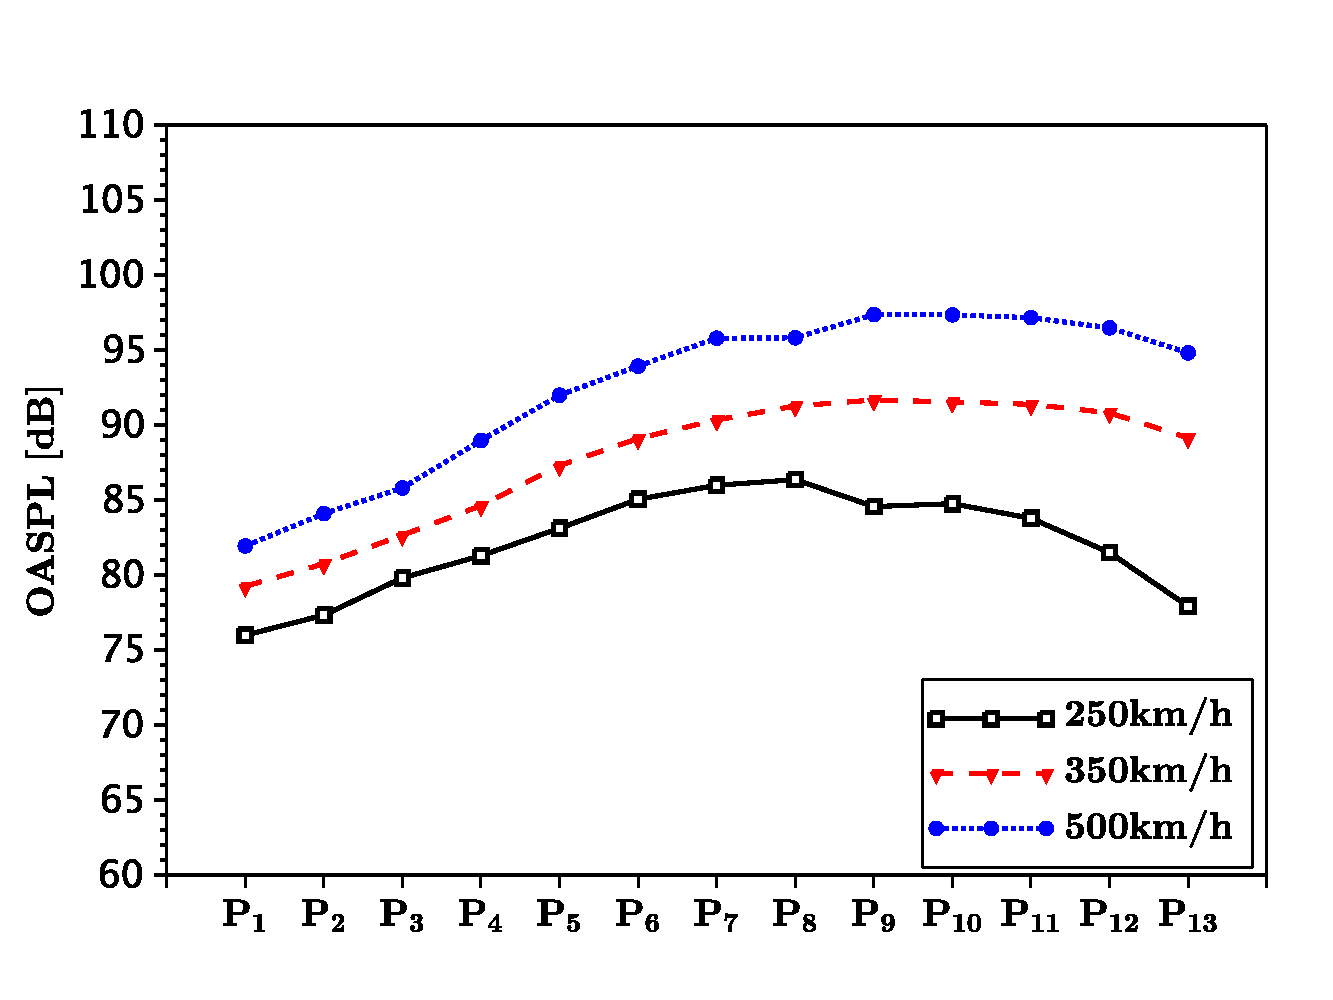
\includegraphics[width=\linewidth]{Figures/oaspl_c.pdf}
  \end{minipage}
  \hfill
  \begin{minipage}[t]{0.46\linewidth}
    \centering
    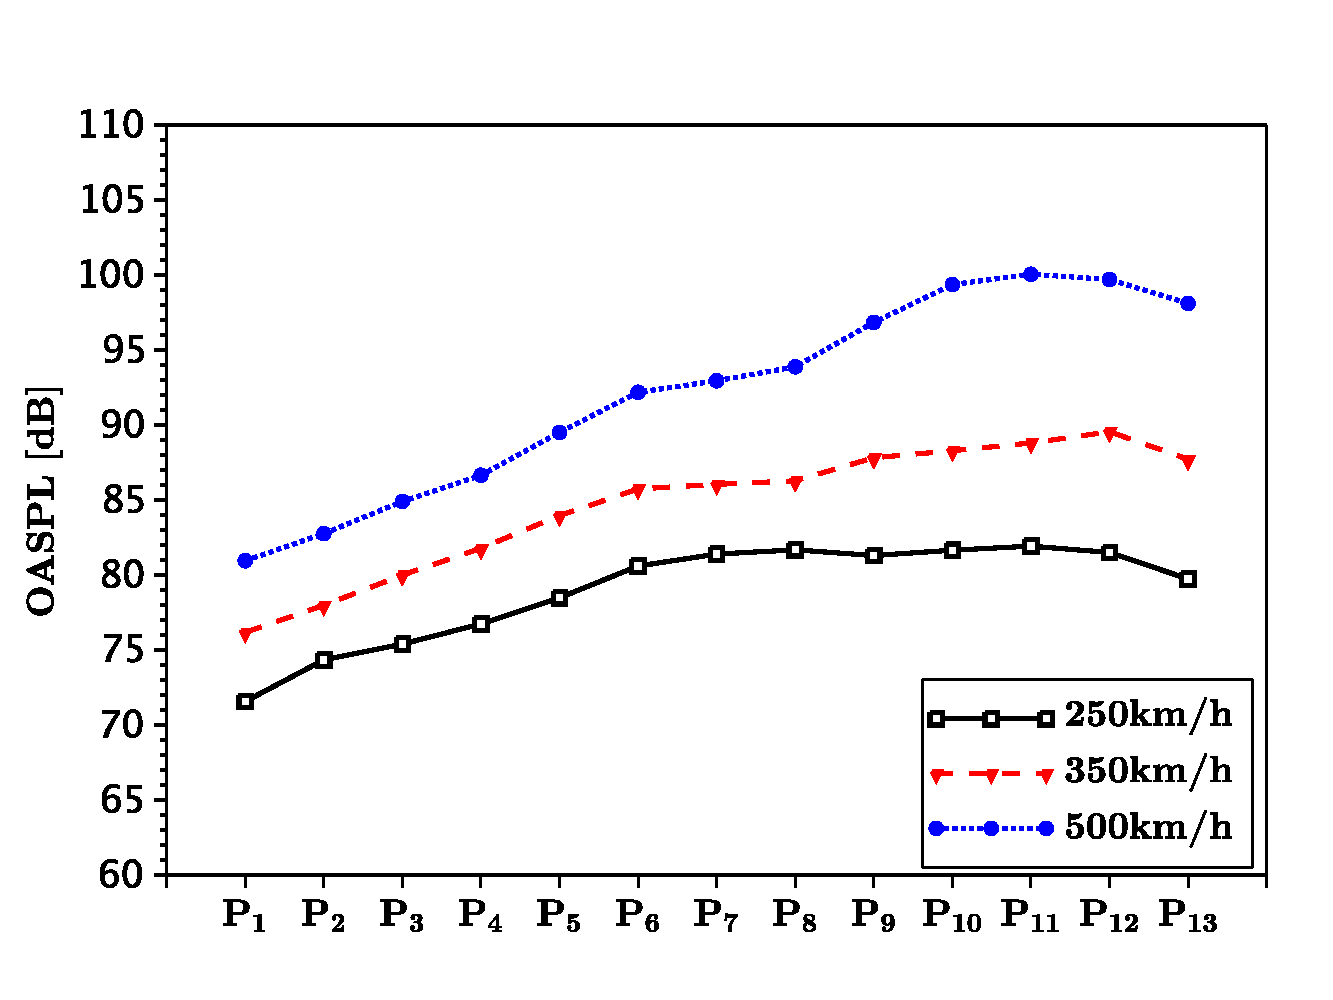
\includegraphics[width=\linewidth]{Figures/oaspl_d.pdf}
  \end{minipage}
  \twofigcaption{fig:ch0-side-by-side}{并列图形排版样例}{Example of Side-by-Side Figures}
\end{figure}

\figref{fig:ch0-side-by-side} 使用 \texttt{minipage} 完成并列排版。
当两幅图共享一个总标题时，可使用这种方式；如果每幅图都需要独立编号，建议拆成两个独立的 \texttt{figure} 环境。

\section{表格排版}

本模板提供 \verb|\twotabcaption{label}{中文题名}{English title}| 用于生成中英文表题。
表题应置于表格上方，正文中使用 \verb|\tabref{label}| 引用。

\subsection{三线表}

文本测试A

\begin{table}[H]
  \centering
  \twotabcaption{tab:ch0-booktabs}{三线表样例}{Example of a Three-Line Table}
  \begin{tabular}{lccc}
    \toprule
    方法 & 准确率（\%） & 召回率（\%） & F1 值 \\
    \midrule
    Baseline & 85.2 & 84.1 & 0.846 \\
    Method A & 89.7 & 88.9 & 0.893 \\
    Proposed & \textbf{92.1} & \textbf{91.5} & \textbf{0.918} \\
    \bottomrule
  \end{tabular}
\end{table}

\tabref{tab:ch0-booktabs} 展示了推荐的三线表格式。
论文中应尽量避免过多竖线，以保持表格简洁。

\subsection{复杂表格}
\begin{table}[H]
  \centering
  \twotabcaption{tab:ch0-complex}{合并单元格与自动换行表格样例}{Example of Merged Cells and Auto-Wrapping Columns}
  \begin{tabularx}{\textwidth}{llXc}
    \toprule
    类别 & 指标 & 说明 & 是否必需 \\
    \midrule
    \multirow{2}{*}{图形} & 分辨率 & 位图图片应保证在最终 PDF 中清晰可辨。 & 是 \\
    & 题名 & 图题使用中英文双语标题，并位于图片下方。 & 是 \\
    \midrule
    \multirow{2}{*}{表格} & 宽度 & 宽表格可使用 \texttt{tabularx} 自动分配列宽。 & 否 \\
    & 表注 & 表内说明应简明，必要时可在正文中解释。 & 否 \\
    \bottomrule
  \end{tabularx}
\end{table}

\tabref{tab:ch0-complex} 同时展示了 \verb|\multirow|、\verb|\makecell| 可配合使用的复杂表格场景。
若单元格内容较长，优先使用 \texttt{tabularx} 或 \texttt{p\{...\}} 列类型控制宽度。

\section{公式排版}

公式应使用标准数学环境，并通过 \verb|\label| 设置标签。
引用公式时建议使用模板提供的 \verb|\equref{label}|。

\subsection{单行公式}
以分类任务中的交叉熵损失为例，可写为
\begin{equation}
  \mathcal{L}(\theta)
  = - \frac{1}{N}\sum_{i=1}^{N}\sum_{k=1}^{K} y_{ik}\log p_{ik}
  \label{eq:ch0-loss}
\end{equation}

如 \equref{eq:ch0-loss} 所示，带编号公式适合放置正文中需要引用的重要定义。

\subsection{多行公式}
循环模型中的状态更新和输出计算可写为
\begin{align}
  h_t &= \sigma(W_x x_t + W_h h_{t-1} + b), \label{eq:ch0-state} \\
  \hat{y}_t &= \operatorname{softmax}(W_o h_t). \label{eq:ch0-output}
\end{align}

\equref{eq:ch0-state} 和 \equref{eq:ch0-output} 展示了多行公式的编号方式。
如果多行推导只需要一个编号，可使用 \texttt{aligned} 放在 \texttt{equation} 环境内部。

\subsection{分段函数与矩阵}
分段函数和矩阵经常同时出现在数学定义中，例如
\begin{equation}
  g(x)=
  \begin{cases}
    0, & x < 0, \\
    x, & 0 \le x < 1, \\
    1, & x \ge 1,
  \end{cases}
  \qquad
  A =
  \begin{bmatrix}
    1 & 0 & 0 \\
    0 & 1 & 0 \\
    0 & 0 & 1
  \end{bmatrix}.
  \label{eq:ch0-piecewise}
\end{equation}

\equref{eq:ch0-piecewise} 展示了分段函数和矩阵的常见写法。

\section{算法伪代码}

计算机类论文常需要给出算法步骤。本文档在 \texttt{main.tex} 中加载了 \texttt{algorithm} 和 \texttt{algorithmic} 宏包，可以直接使用如下环境。

\begin{algorithm}[H]
  \caption{样例训练流程}
  \label{alg:ch0-training}
  \begin{algorithmic}[1]
    \REQUIRE Training set $\mathcal{D}$, learning rate $\eta$, maximum epoch $T$
    \ENSURE Model parameters $\theta$
    \STATE Initialize parameters $\theta$
    \FOR{$t = 1$ to $T$}
      \STATE Sample a mini-batch $\mathcal{B}$ from $\mathcal{D}$
      \STATE Compute loss $\mathcal{L}(\theta)$ by \equref{eq:ch0-loss}
      \STATE Update $\theta \leftarrow \theta - \eta \nabla_{\theta}\mathcal{L}(\theta)$
    \ENDFOR
    \RETURN $\theta$
  \end{algorithmic}
\end{algorithm}

算法~\ref{alg:ch0-training} 展示了带行号的伪代码。
若需要中文关键字，可在导言区重定义相应命令。

\section{引用、链接与交叉引用}

参考文献引用可使用两种方式：
上标引用适合放在句末，例如已有研究讨论了神经网络轻量化问题\upcite{guo_2023_research}；
正文引用适合作为句子成分，例如文献 \inlinecite{thakkar_2018_performance} 给出了系统性能评测案例。
多篇文献可写在同一条引用命令中，例如区块链平台相关研究\upcite{zheng_2019_nutbaas,thakkar_2018_performance}。

交叉引用建议统一使用模板命令：
\begin{itemize}
  \item 图引用：\verb|\figref{fig:ch0-pdf}|，效果为 \figref{fig:ch0-pdf}。
  \item 表引用：\verb|\tabref{tab:ch0-complex}|，效果为 \tabref{tab:ch0-complex}。
  \item 公式引用：\verb|\equref{eq:ch0-loss}|，效果为 \equref{eq:ch0-loss}。
  \item 算法引用：当前模板未单独封装算法引用命令，可写作“算法~\ref{alg:ch0-training}”。
\end{itemize}
|。
脚注示例如此处所示\footnote{脚注用于补充说明，不宜放置过长的正文内容。}。

\subsection{字体、字号与强调}

模板预定义了常用中文字体命令。正式论文中通常不需要手动切换字体；只有在展示样式、术语强调或特殊说明时才建议使用。
需要注意的是，Windows 常用中文字体多数只有常规字重，没有独立的粗体字形。
因此 \verb|\bfseries| 或 \verb|\textbf| 对宋体、黑体、楷体、仿宋等中文字体未必产生真正加粗效果；模板中的黑体标题主要依靠“黑体”本身的笔画风格，而不是额外叠加粗体。
若需要强调中文内容，建议优先使用黑体、调整标题层级或通过文字表述强调，不建议依赖中文伪粗体。

\begin{table}[H]
  \centering
  \twotabcaption{tab:ch0-fonts}{字体与强调样例}{Examples of Fonts and Emphasis}
  \begin{tabular}{lll}
    \toprule
    命令 & 显示效果 & 使用建议 \\
    \midrule
    \verb|\song| & {\song 宋体文字示例} & 正文默认字体 \\
    \verb|\hei| & {\hei 黑体文字示例} & 标题或强调场景 \\
    \verb|\kai| & {\kai 楷体文字示例} & 摘要、题签或引用语 \\
    \verb|\fs| & {\fs 仿宋文字示例} & 特殊文书类内容 \\
    \verb|\textbf| & \textbf{加粗文字示例} & 主要用于英文、数字或有粗体字重的字体 \\
    \verb|\textit| & \textit{Italic text example} & 英文斜体或变量说明 \\
    \bottomrule
  \end{tabular}
\end{table}

\subsection{列表环境}

无序列表适合列出并列事项：
\begin{itemize}
  \item 图题位于图下方，表题位于表上方。
  \item 图表应使用中英文双语标题。
  \item 公式、图、表、算法均应使用标签进行交叉引用。
\end{itemize}

有序列表适合描述步骤：
\begin{enumerate}
  \item 在 \texttt{main.tex} 中填写论文元信息。
  \item 在各章文件中撰写正文内容。
  \item 使用 \texttt{latexmk -xelatex main.tex} 完成编译。
\end{enumerate}

\section{图形排版}

本模板提供 \verb|\twofigcaption{label}{中文题名}{English title}| 用于生成中英文图题。
图题应置于图形下方，正文中使用 \verb|\figref{label}| 引用。

\subsection{外部图片}
\begin{figure}[H]
  \centering
  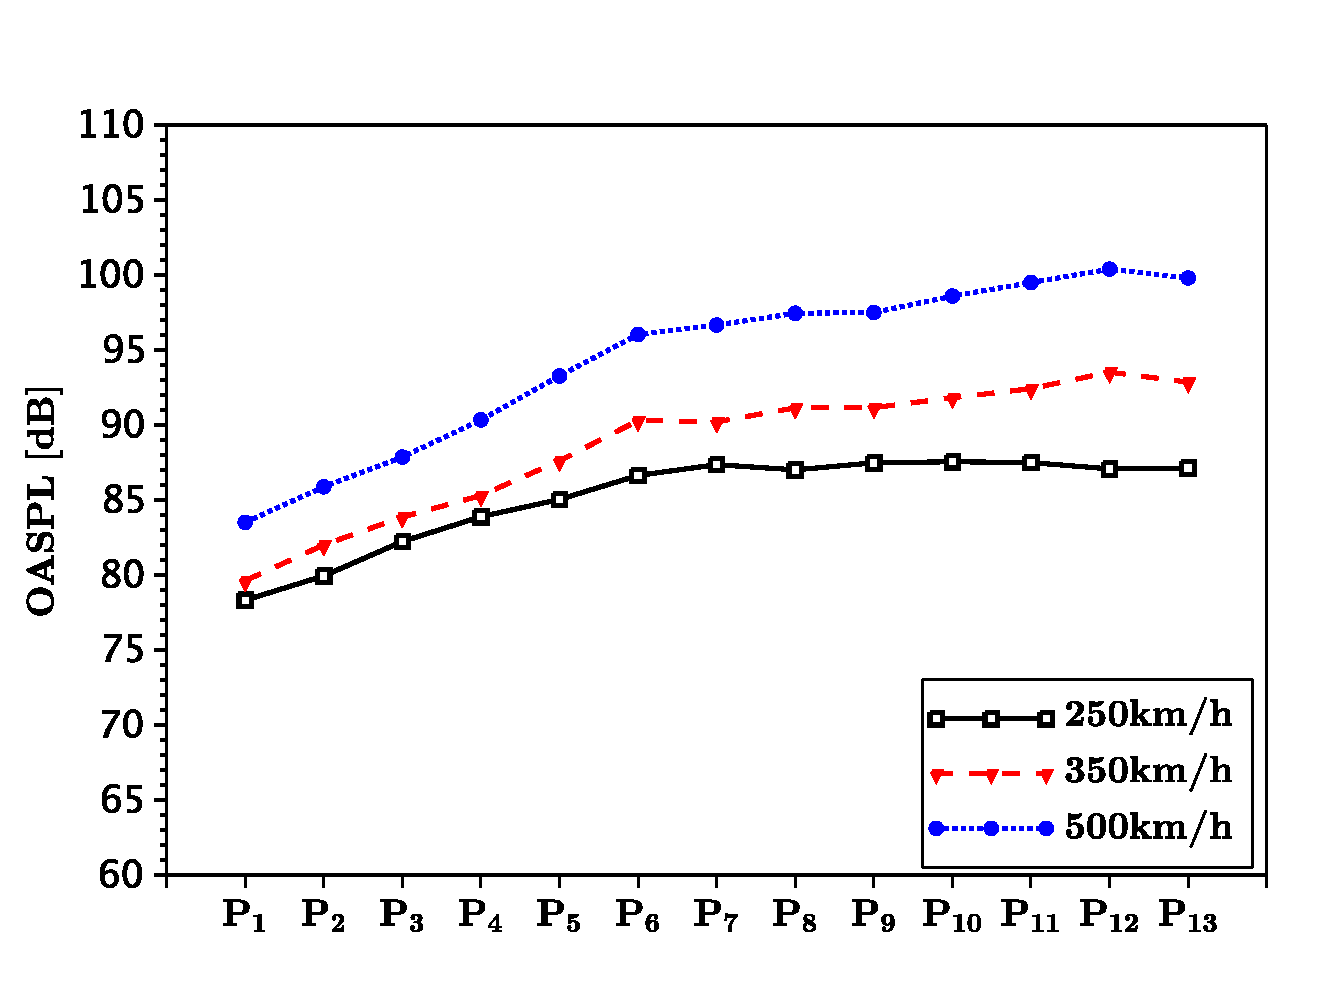
\includegraphics[width=0.55\textwidth]{Figures/oaspl_a.pdf}
  \twofigcaption{fig:ch0-cover}{外部图片插入样例}{Example of Including an External Image}
\end{figure}

\figref{fig:ch0-cover} 展示了通过 \verb|\includegraphics| 插入图片文件的方式。
正式论文中建议将图片统一放入 \texttt{Figures} 目录，并使用相对路径引用。

\subsection{PDF 或位图图片}
\begin{figure}[H]
  \centering
  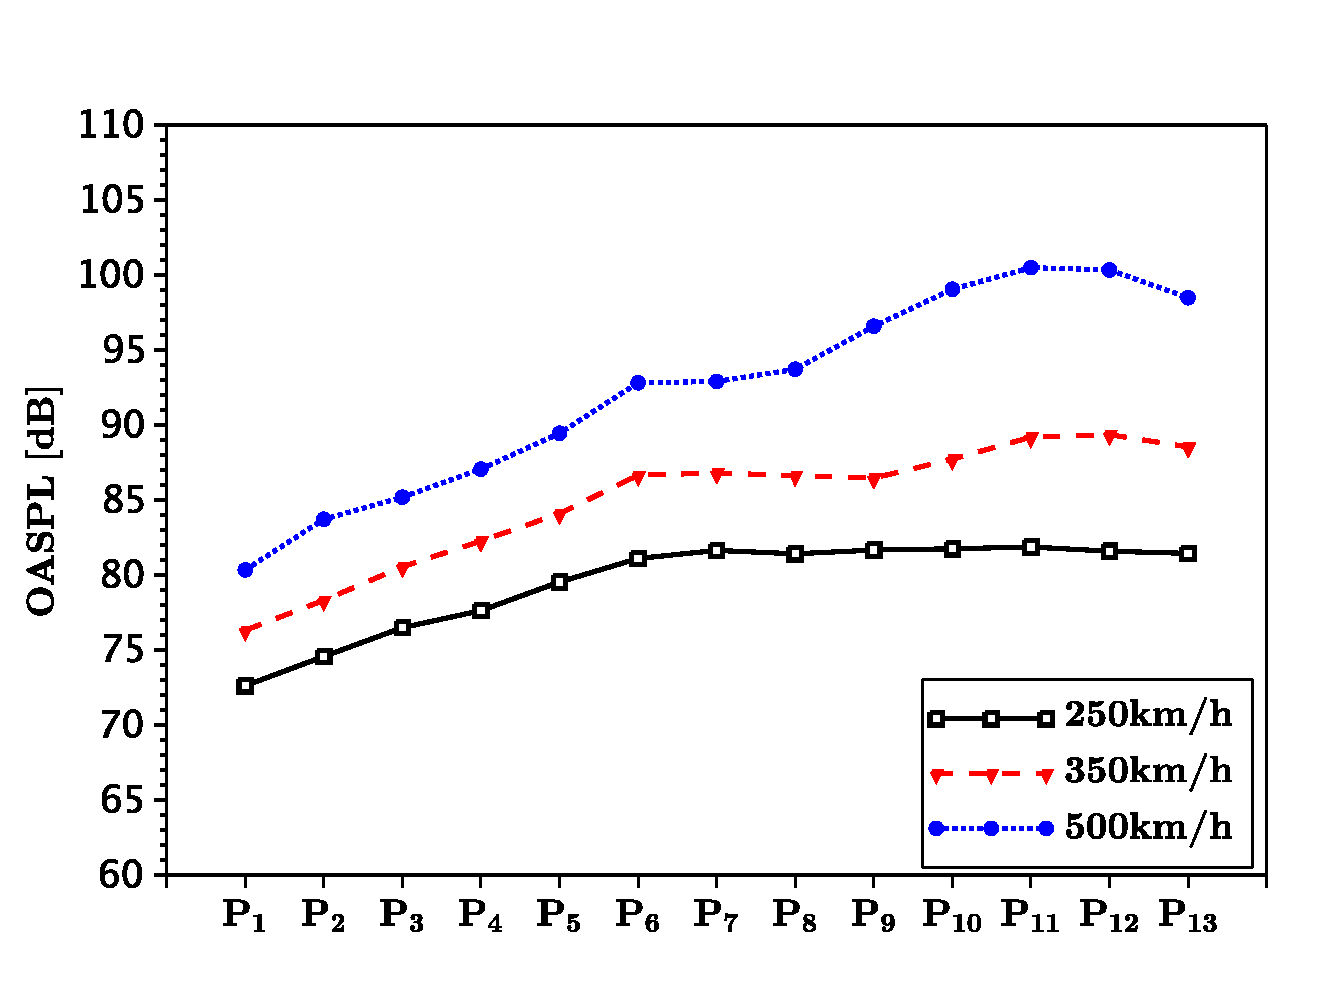
\includegraphics[width=0.55\textwidth]{Figures/oaspl_b.pdf}
  \twofigcaption{fig:ch0-pdf}{PDF 图片插入样例}{Example of Including a PDF Figure}
\end{figure}

PDF、PNG、JPG 等常见图片格式均可通过 \verb|\includegraphics| 插入。
若图片由绘图软件或数据分析程序导出，建议优先使用 PDF 格式以保持较清晰的显示效果。

\subsection{并列图片}
\begin{figure}[H]
  \centering
  \begin{minipage}[t]{0.46\linewidth}
    \centering
    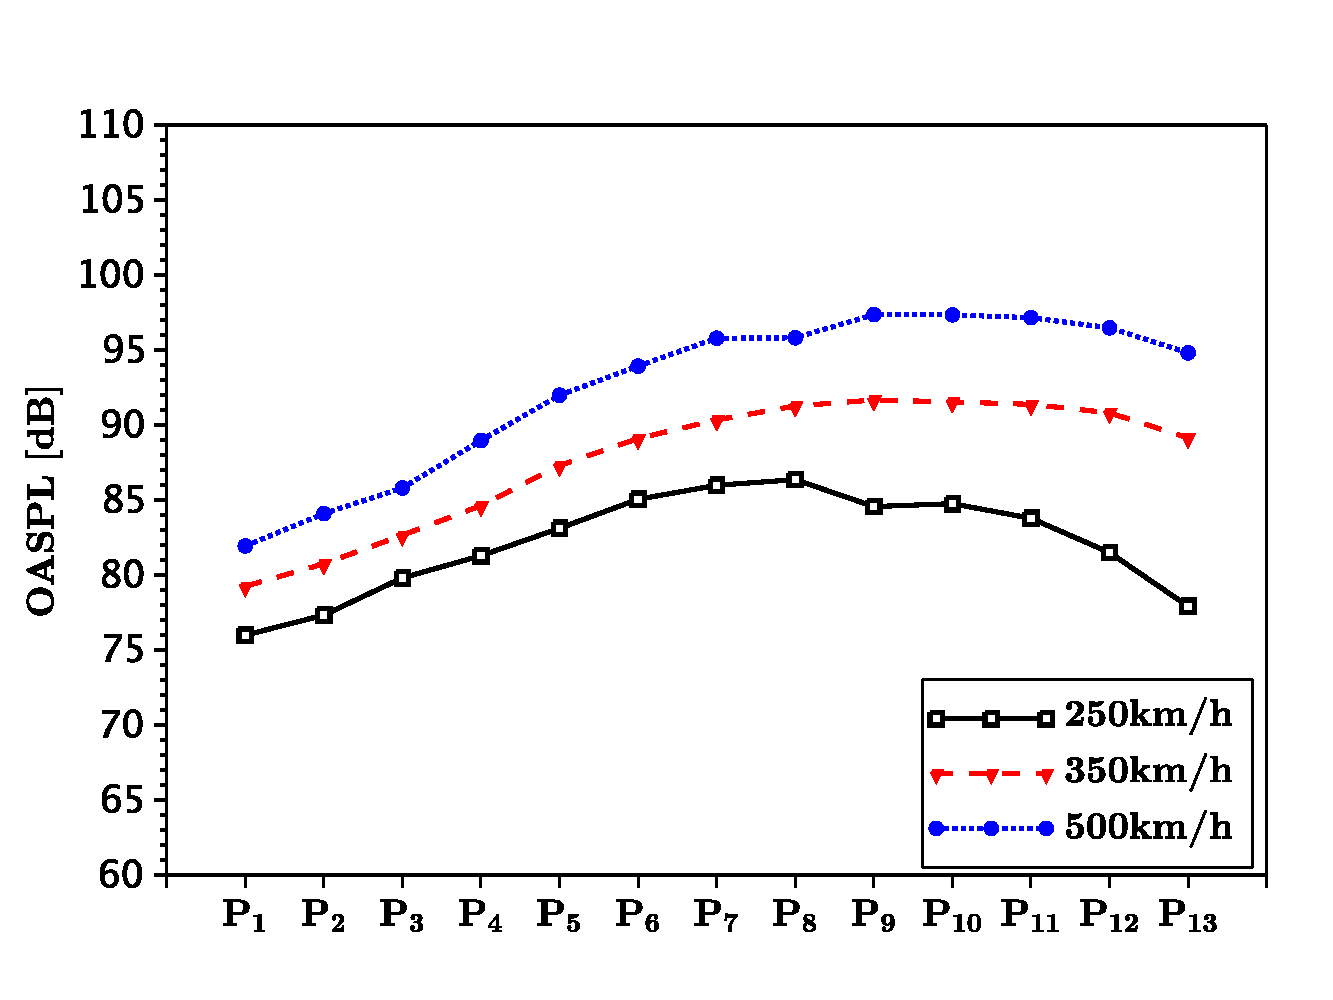
\includegraphics[width=\linewidth]{Figures/oaspl_c.pdf}
  \end{minipage}
  \hfill
  \begin{minipage}[t]{0.46\linewidth}
    \centering
    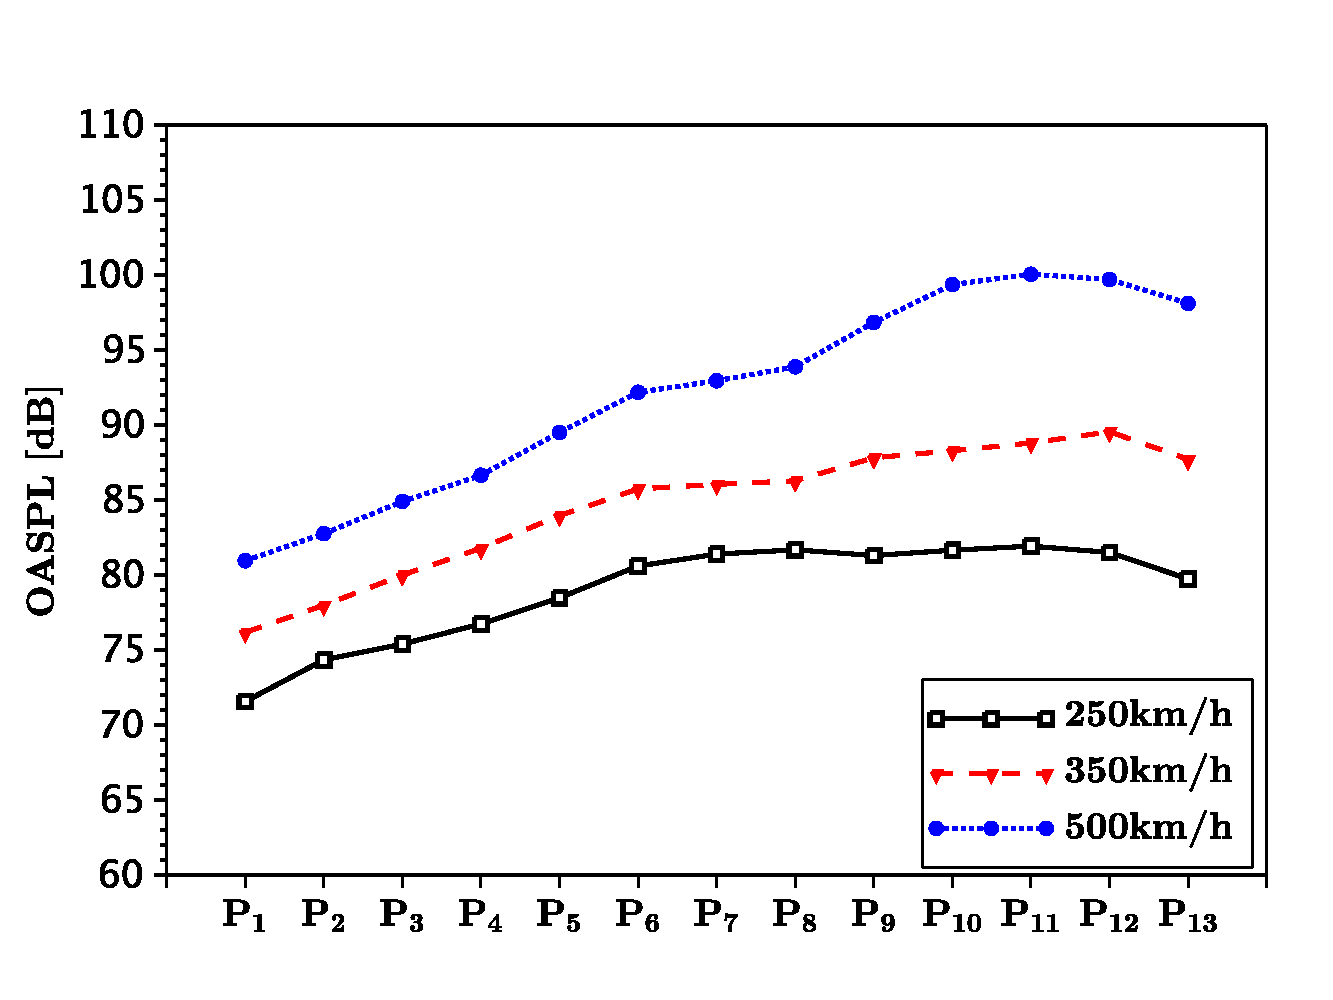
\includegraphics[width=\linewidth]{Figures/oaspl_d.pdf}
  \end{minipage}
  \twofigcaption{fig:ch0-side-by-side}{并列图形排版样例}{Example of Side-by-Side Figures}
\end{figure}

\figref{fig:ch0-side-by-side} 使用 \texttt{minipage} 完成并列排版。
当两幅图共享一个总标题时，可使用这种方式；如果每幅图都需要独立编号，建议拆成两个独立的 \texttt{figure} 环境。

\section{表格排版}

本模板提供 \verb|\twotabcaption{label}{中文题名}{English title}| 用于生成中英文表题。
表题应置于表格上方，正文中使用 \verb|\tabref{label}| 引用。

\subsection{三线表}

文本测试A

\begin{table}[H]
  \centering
  \twotabcaption{tab:ch0-booktabs}{三线表样例}{Example of a Three-Line Table}
  \begin{tabular}{lccc}
    \toprule
    方法 & 准确率（\%） & 召回率（\%） & F1 值 \\
    \midrule
    Baseline & 85.2 & 84.1 & 0.846 \\
    Method A & 89.7 & 88.9 & 0.893 \\
    Proposed & \textbf{92.1} & \textbf{91.5} & \textbf{0.918} \\
    \bottomrule
  \end{tabular}
\end{table}

\tabref{tab:ch0-booktabs} 展示了推荐的三线表格式。
论文中应尽量避免过多竖线，以保持表格简洁。

\subsection{复杂表格}
\begin{table}[H]
  \centering
  \twotabcaption{tab:ch0-complex}{合并单元格与自动换行表格样例}{Example of Merged Cells and Auto-Wrapping Columns}
  \begin{tabularx}{\textwidth}{llXc}
    \toprule
    类别 & 指标 & 说明 & 是否必需 \\
    \midrule
    \multirow{2}{*}{图形} & 分辨率 & 位图图片应保证在最终 PDF 中清晰可辨。 & 是 \\
    & 题名 & 图题使用中英文双语标题，并位于图片下方。 & 是 \\
    \midrule
    \multirow{2}{*}{表格} & 宽度 & 宽表格可使用 \texttt{tabularx} 自动分配列宽。 & 否 \\
    & 表注 & 表内说明应简明，必要时可在正文中解释。 & 否 \\
    \bottomrule
  \end{tabularx}
\end{table}

\tabref{tab:ch0-complex} 同时展示了 \verb|\multirow|、\verb|\makecell| 可配合使用的复杂表格场景。
若单元格内容较长，优先使用 \texttt{tabularx} 或 \texttt{p\{...\}} 列类型控制宽度。

\section{公式排版}

公式应使用标准数学环境，并通过 \verb|\label| 设置标签。
引用公式时建议使用模板提供的 \verb|\equref{label}|。

\subsection{单行公式}
以分类任务中的交叉熵损失为例，可写为
\begin{equation}
  \mathcal{L}(\theta)
  = - \frac{1}{N}\sum_{i=1}^{N}\sum_{k=1}^{K} y_{ik}\log p_{ik}
  \label{eq:ch0-loss}
\end{equation}

如 \equref{eq:ch0-loss} 所示，带编号公式适合放置正文中需要引用的重要定义。

\subsection{多行公式}
循环模型中的状态更新和输出计算可写为
\begin{align}
  h_t &= \sigma(W_x x_t + W_h h_{t-1} + b), \label{eq:ch0-state} \\
  \hat{y}_t &= \operatorname{softmax}(W_o h_t). \label{eq:ch0-output}
\end{align}

\equref{eq:ch0-state} 和 \equref{eq:ch0-output} 展示了多行公式的编号方式。
如果多行推导只需要一个编号，可使用 \texttt{aligned} 放在 \texttt{equation} 环境内部。

\subsection{分段函数与矩阵}
分段函数和矩阵经常同时出现在数学定义中，例如
\begin{equation}
  g(x)=
  \begin{cases}
    0, & x < 0, \\
    x, & 0 \le x < 1, \\
    1, & x \ge 1,
  \end{cases}
  \qquad
  A =
  \begin{bmatrix}
    1 & 0 & 0 \\
    0 & 1 & 0 \\
    0 & 0 & 1
  \end{bmatrix}.
  \label{eq:ch0-piecewise}
\end{equation}

\equref{eq:ch0-piecewise} 展示了分段函数和矩阵的常见写法。

\section{算法伪代码}

计算机类论文常需要给出算法步骤。本文档在 \texttt{main.tex} 中加载了 \texttt{algorithm} 和 \texttt{algorithmic} 宏包，可以直接使用如下环境。

\begin{algorithm}[H]
  \caption{样例训练流程}
  \label{alg:ch0-training}
  \begin{algorithmic}[1]
    \REQUIRE Training set $\mathcal{D}$, learning rate $\eta$, maximum epoch $T$
    \ENSURE Model parameters $\theta$
    \STATE Initialize parameters $\theta$
    \FOR{$t = 1$ to $T$}
      \STATE Sample a mini-batch $\mathcal{B}$ from $\mathcal{D}$
      \STATE Compute loss $\mathcal{L}(\theta)$ by \equref{eq:ch0-loss}
      \STATE Update $\theta \leftarrow \theta - \eta \nabla_{\theta}\mathcal{L}(\theta)$
    \ENDFOR
    \RETURN $\theta$
  \end{algorithmic}
\end{algorithm}

算法~\ref{alg:ch0-training} 展示了带行号的伪代码。
若需要中文关键字，可在导言区重定义相应命令。

\section{引用、链接与交叉引用}

参考文献引用可使用两种方式：
上标引用适合放在句末，例如已有研究讨论了神经网络轻量化问题\upcite{guo_2023_research}；
正文引用适合作为句子成分，例如文献 \inlinecite{thakkar_2018_performance} 给出了系统性能评测案例。
多篇文献可写在同一条引用命令中，例如区块链平台相关研究\upcite{zheng_2019_nutbaas,thakkar_2018_performance}。

交叉引用建议统一使用模板命令：
\begin{itemize}
  \item 图引用：\verb|\figref{fig:ch0-pdf}|，效果为 \figref{fig:ch0-pdf}。
  \item 表引用：\verb|\tabref{tab:ch0-complex}|，效果为 \tabref{tab:ch0-complex}。
  \item 公式引用：\verb|\equref{eq:ch0-loss}|，效果为 \equref{eq:ch0-loss}。
  \item 算法引用：当前模板未单独封装算法引用命令，可写作“算法~\ref{alg:ch0-training}”。
\end{itemize}

%!TEX root = ./main.tex
\chapter{绪论}
\label{chap:introduction}

\section{研究背景}

今天，计算机技术和互联网络的飞速发展把社会的信息化进程推向了一个全新的阶段，信息的传递与交流已经成为整个现代社会生活运作的重要基础，电子可读文本大量涌现并成为网络时代主要的信息载体和人们的生活中不可缺的一部分。随着信息化进代的来临，自然语言处理技术已逐渐成为一项大从的迫切需求，计算语言学的研究也越来越受到人们的重视。

自然语言分析技术（Natural Language Parsing）一直是计算语言学领域一个基础性的研究课题。大部分自然语言处理系统，包括机器翻译，文本理解，信息的检索与过滤，语音识别与合成，都毫无疑问地会从高质量的分析技术中受益。从科学的观点来看，计算机的自然语言分析过程是对人类语言理解过程的模拟：即根据一定的语言知识，通常是一具由规则、树或图组成的形式文法系统，将输入句子的一维线性结构赋予某种二维平面结构解释；从人工工智能研究的角度来讲，这是一个基于推理的问题求解过程，分析方法则对应了其推理控制策略。~\cite{guo_2023_research,thakkar_2018_performance,zheng_2019_nutbaas}

Testing测试12345章节~\upcite{guo_2023_research}

\subsection{结构歧义}

然而与形式语言的分析相比，应用计算机进行自然语言的结构分析却远非一件容易的工作。

\subsubsection{测试AA}

然而与形式语言的分析相比，应用计算机进行自然语言的结构分析却远非一件容易的工作。

\input{chapter2}
\input{chapter3}
\input{chapter4}
\input{chapter5}
\input{chapter6}

\backmatter

\addcontentsline{toc}{chapter}{参考文献}
\nocite{guo_2023_research}
\bibliography{references}

\chapter{攻读博士学位期间取得的学术成果}
\begin{enumerate}
  \item 第一作者. 示例论文题名[J]. 示例期刊，20xx，1（1）：1-10. （检索情况）（对应论文第一章）
  \item 第一排序. 示例专利题名：中国，XXXXXXXXX[P]. 20xx-xx-xx. （对应论文第二章）
\end{enumerate}

\input{thanks}

\end{document}
